\section{Error Analysis}\label{s:simulation}
We now focus on computing the newly obtained MGF expressions numerically. To highlight the errors of the Caputo-Fabrizio MGF, moments of various orders with different parameter configurations will be computed. However, before computing these errors involving explicit distributions, we first focus on the expression \[ E(x, \alpha) = x^\alpha - \displaystyle \frac{x^{n+1} }{(1 - \beta)x + \beta}\] which is of great importance in order to fully comprehend the errors discussed in section \ref{ss:accuracy_analysis}

\subsection{Analysing a particular error term of interest of the Caputo-Fabrizio MGF}
We explicitly focus on the term 
\begin{equation}\label{def:error} 
    E(x, \alpha) = x^\alpha - \displaystyle \frac{x^{n+1} }{(1 - \beta)x + \beta}
\end{equation}
 for simplicity. The expression we analyse, denoted \(E(x, \alpha)\) is not the same as the expression obtained in theorem \ref{t: MGF_inaccurate}. Yet, it is the part of the expression that involves the order term \(\alpha\) and is thus of great interest. What is more, considering the result obtained in theorem \ref{t: MGF_inaccurate}, it is easy to see that \(\leftindex_{CF}{M}_X^{(\alpha)}\) is accurate \(\iff x^\alpha = \displaystyle \frac{x^{n+1} }{(1 - \beta)x + \beta}\). Thus, we consider the function \(E(x, \alpha)\), to be the function of their differences and analyse when this function equals zero. Plotting this expression for different orders of \(\alpha\), we obtain the following figure:
\begin{figure}[H]
    \centering
    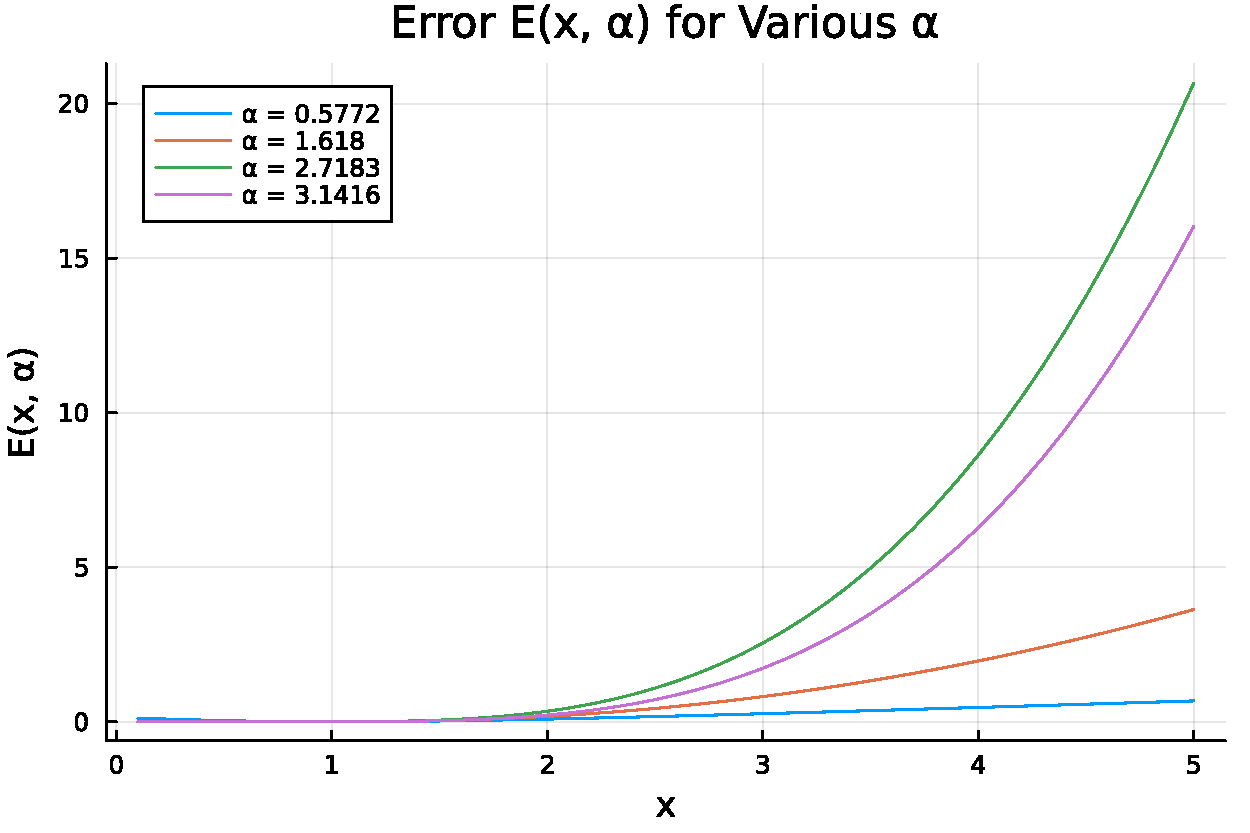
\includegraphics[width=0.7\textwidth]{figures/error_plot.pdf}
    \caption{Error of Caputo-Fabrizio MGF}
    \label{fig:error_MGF}
\end{figure}
It can be observed from figure \ref{fig:error_MGF} above that, in general for greater orders \(\alpha\), the error tends to increase. However, the greatest order of \(\alpha\) does not provide the greatest error. Instead it is the second greatest order of \(\alpha\) that does so. This may be explained by the fact that for values of \(\alpha\), being exactly in the middle of two integers, the value of \((1 - \beta)x + \beta\) will be the greatest. As a result, the fraction of error term \ref{def:error} becomes small, thus the error tends to increase.

This hypothesis is indeed confirmed in the following figure, which focuses on the growth rate of the error, for a fixed value of \(x\) and an increasing order \(\alpha\).

\begin{figure}[H]
    \centering
    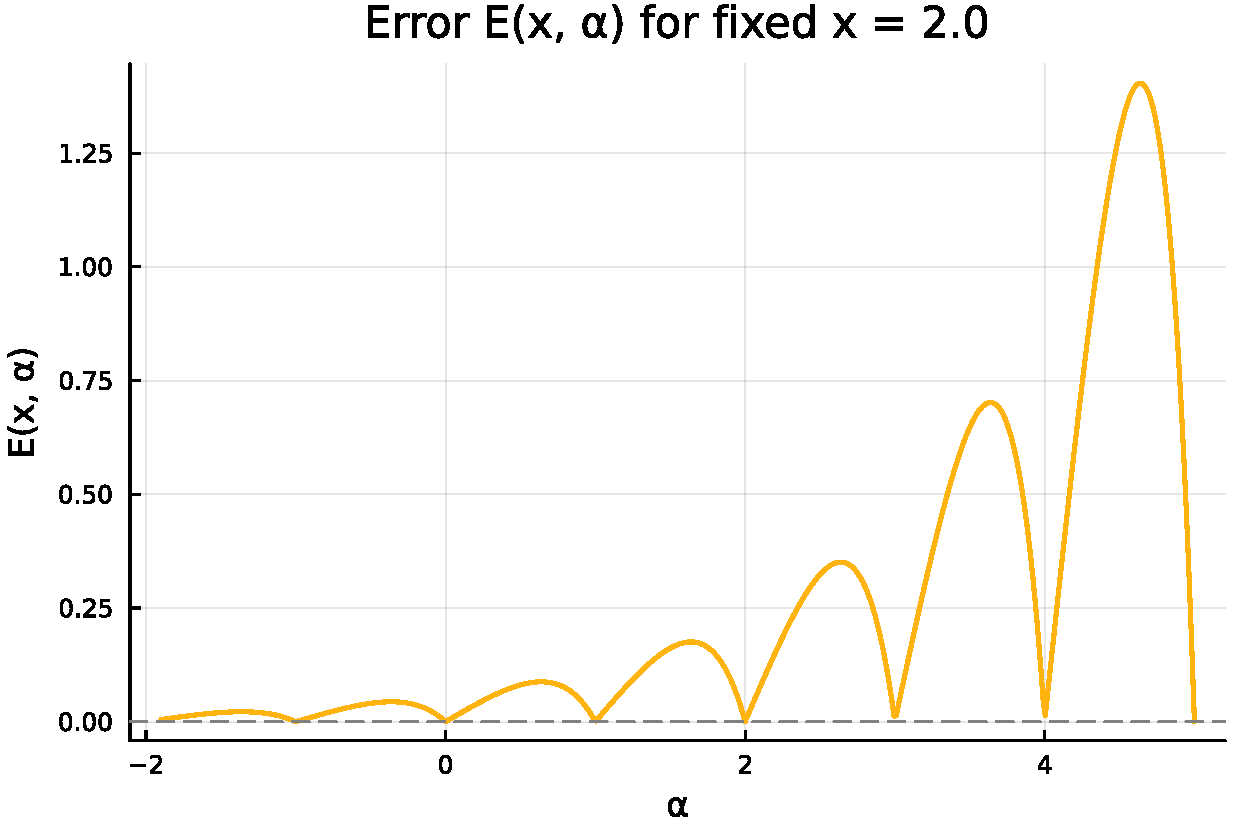
\includegraphics[width=0.7\textwidth]{figures/error_plot_fixed_x.pdf}
    \caption{Error of Caputo-Fabrizio MGF, for fixed x}
    \label{fig:error_MGF_fixed_x}
\end{figure}
Figure \ref{fig:error_MGF_fixed_x} indeed seems to indicate that for some \(\alpha \in (a, b)\), where \(a, b \in \mathbb{Z}\) are consecutive integers that \(E(x, \alpha)\) attains it maximum value for some \(\alpha\) 'slightly greater' than \(\frac{a + b}{2}\). Figure \ref{fig:error_MGF_fixed_x} also reveals that the approximation error is considerably smaller for negative fractional moments compared to the positive ones. This suggests that, when negative moments are well-defined, the Caputo-Fabrizio MGF may still offer reasonable accuracy, despite its known limitations.

Note that within each subsequent integer interval, the function \(E(x, \alpha)\) appears to be concave. Thus, as is supported by figure \ref{fig:error_MGF_fixed_x}, it is only possible to obtain local maxima. Ideally, one would aim to analytically determine the optimal order \(\hat{\alpha}\) such that minimizes \(E(x, \hat{\alpha})\). However, due to the concavity of \(E(x, \alpha)\), such analytical minimization is not feasible. Figure \ref{fig:error_MGF_fixed_x} seems to suggest that the order of \(\alpha\) near integer orders yields smaller approximation errors, which makes sense intuitively. However, the latter is not rigorous evidence. Therefore, in the following section, we will analyse the numerical approximation errors of the Caputo-Fabrizio MGF by computing moments of fractional order for different distributions and various orders \(\alpha\).

\subsection{Practical Issues}
Computing fractional moments of a specific distribution poses some difficulties. In the first place, we want to compute the moment of fractional order \(\alpha\) for a random variable \(X\). Official packages to compute raw moments of fractional order do not exist yet, thus these methods will have to be created first. In order to accomplish the desired result, we directly compute \(\int_{-\infty}^{\infty} x^\alpha  f_X(x) dx\). If the support of the random variable is infinite, this integral is often not numerically well defined or takes too long to compute. Thus, in such cases we use a bounded support \((-100, 100)\) which provides a sufficiently accurate approximation. What is more, for many fractional orders \(\alpha\) in combination with negative values of \(x\), \(x^\alpha\) is of complex form. If a distribution has a support which contains negative values, it is possible to compute the complex or absolute moment of fractional order, which avoids any numerical issues. This approach, however, lacks interpretability, as the intuition behind absolute and complex moments is harder to grasp.

It now remains to compute the fractional moment using the Caputo-Fabrizio MGF. Unfortunately, it is rather difficult to compute fractional derivatives of an MGF expression numerically. The reason is, that programming packages often take (fractional) derivatives on a certain point \(x\) rather than over the entire function. Thus, we simply use the result obtained in theorem \ref{t: MGF_inaccurate}. That is, instead of the moment of order \(\alpha\), the Caputo-Fabrizio MGF computes the moment of order \(n+1\) divided by some variables dependent on \(\alpha\). More explicitly, we compute \(\leftindex_{CF}{M}_X^{(\alpha)}(0) = \displaystyle \int_{-\infty}^{\infty}  \frac{x^{n+1} }{(1 - \beta)x + \beta} f_X(x) dx\). Throughout the rest of the thesis, this is the expression that is being computed whenever values of the Caputo-Fabrizio MGF are discussed. This integral faces the same problems as the aforementioned integral including \(x^\alpha\). What is more, for specific values of \(x\) and \(\beta\), the denominator tends to go towards zero, which is numerically unstable. Thus, in such cases, we add a small \(\epsilon > 0\) in order to avoid this issue.

\subsection{Accuracy Analysis}\label{ss:accuracy_analysis}
For this accuracy analysis we will compute fractional moments based on different parameter values and orders of \(\alpha\). We set \(\alpha \in [0, 5]\) with steps of 0.01. This yields 500 different fractional moments per parameter-configuration. We consider three distributions, namely the Exponential, Normal and Poisson distribution. This selection allows us to cover both continuous and discrete distributions, and distributions with negative and positive supports. 

\subsubsection{Computing fractional moments for various distributions}
Before analysing the errors of the Caputo-Fabrizio MGF, we first compare the values obtained by each method. Specifically, we compute:
\begin{itemize}
    \item \textbf{Theoretical values:} \(\displaystyle \int_{-\infty}^{\infty} x^\alpha  f_X(x) dx\), which has been shown to coincide with the Riemann-Liouville and Grünwald-Letnikov MGFs.
    \item \textbf{Caputo-Fabrizio MGF:} \(\displaystyle \int_{-\infty}^{\infty}  \frac{x^{n+1} }{(1 - \beta)x + \beta} f_X(x) dx\)
    \item \textbf{Complex moment generating function (CMGF):} defined as in equation \ref{eq:hansen} in section \ref{ss:methodology_introduction}, which computation is given in algorithm \ref{alg:cmgf_dist}. In this case, \(\xi = 0\).
    \item \textbf{Empirical values:} \(\displaystyle\mathbb{E}[|X|^\alpha] \approx \frac{1}{n} \sum_{i=1}^{n} |x_i|^\alpha\). Where \(\{x_i\}_{i=1}^{n}\) are simulated samples and \(n = 1.000.000\).
\end{itemize}

For the Poisson, Exponential and Normal distribution, we obtain the following figures: 
\begin{figure}[H]
    \centering
    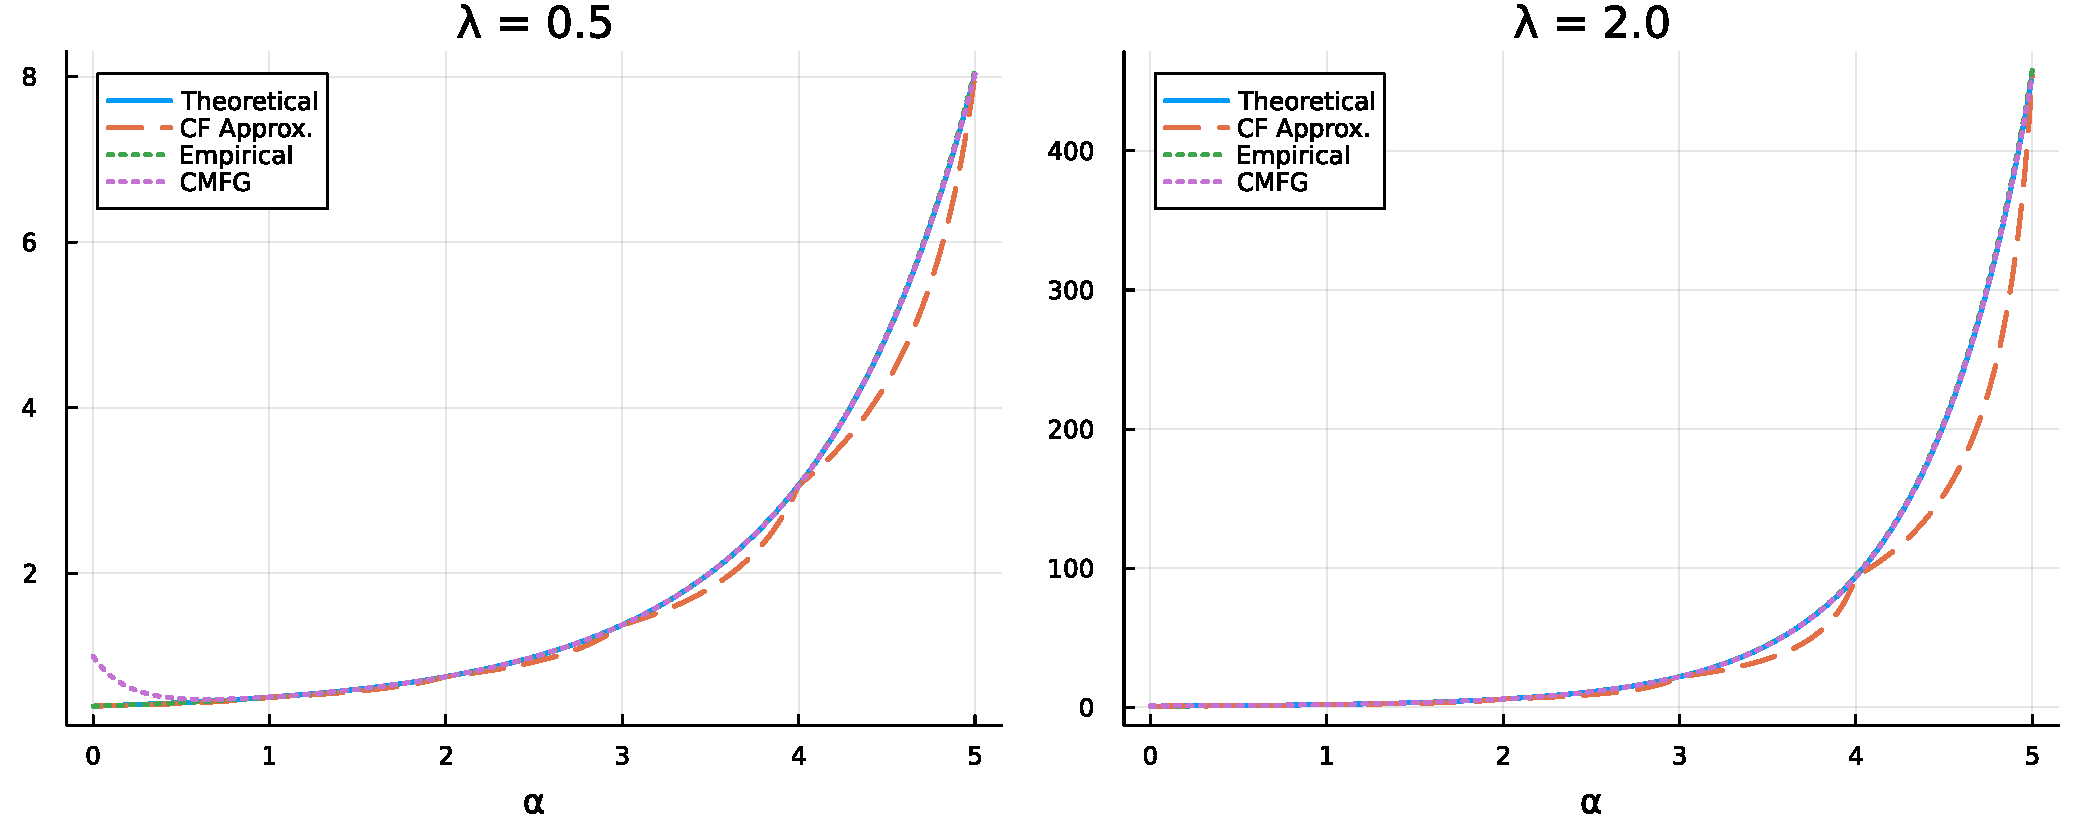
\includegraphics[width=1.1\textwidth]{figures/value_comparison_poisson.pdf}
    \caption{Comparison of different fractional moments for the Poisson Distribution}
    \label{fig:poisson_plot_values}
\end{figure}

\begin{figure}[H]
    \centering
    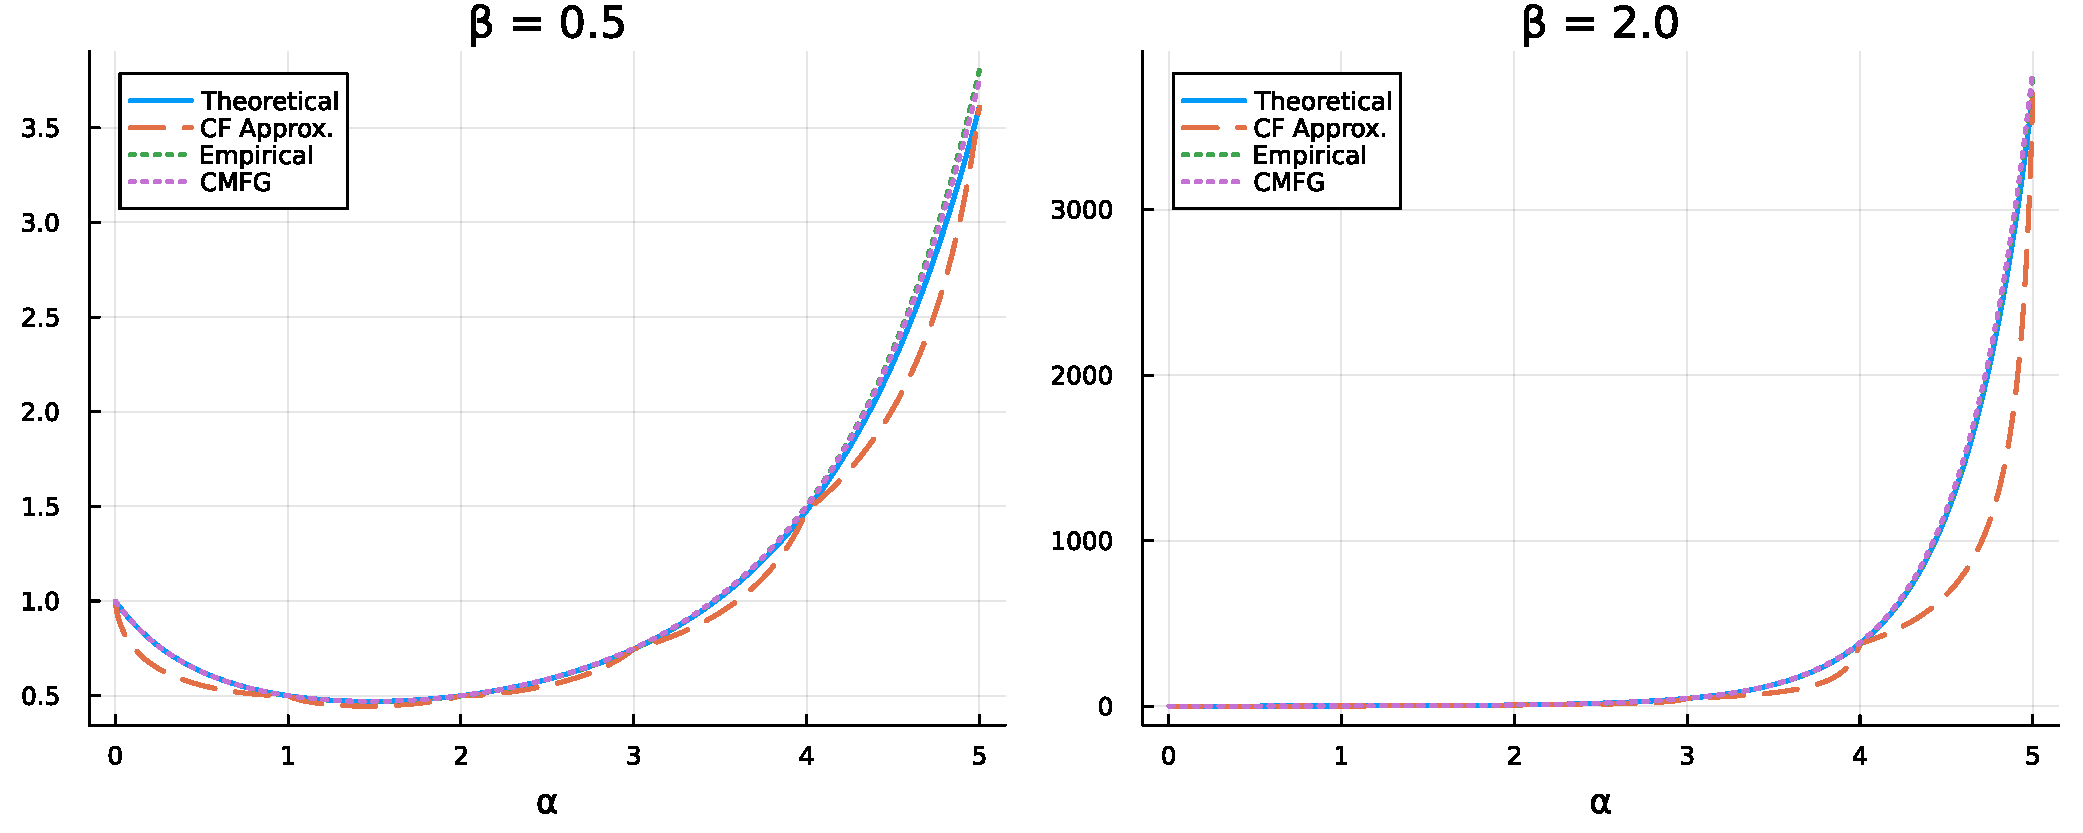
\includegraphics[width=1.1\textwidth]{figures/value_comparison_exponential.pdf}
    \caption{Comparison of different fractional moments for the Exponential Distribution}
    \label{fig:exponential_plot_values}
\end{figure}

\begin{figure}[H]
    \centering
    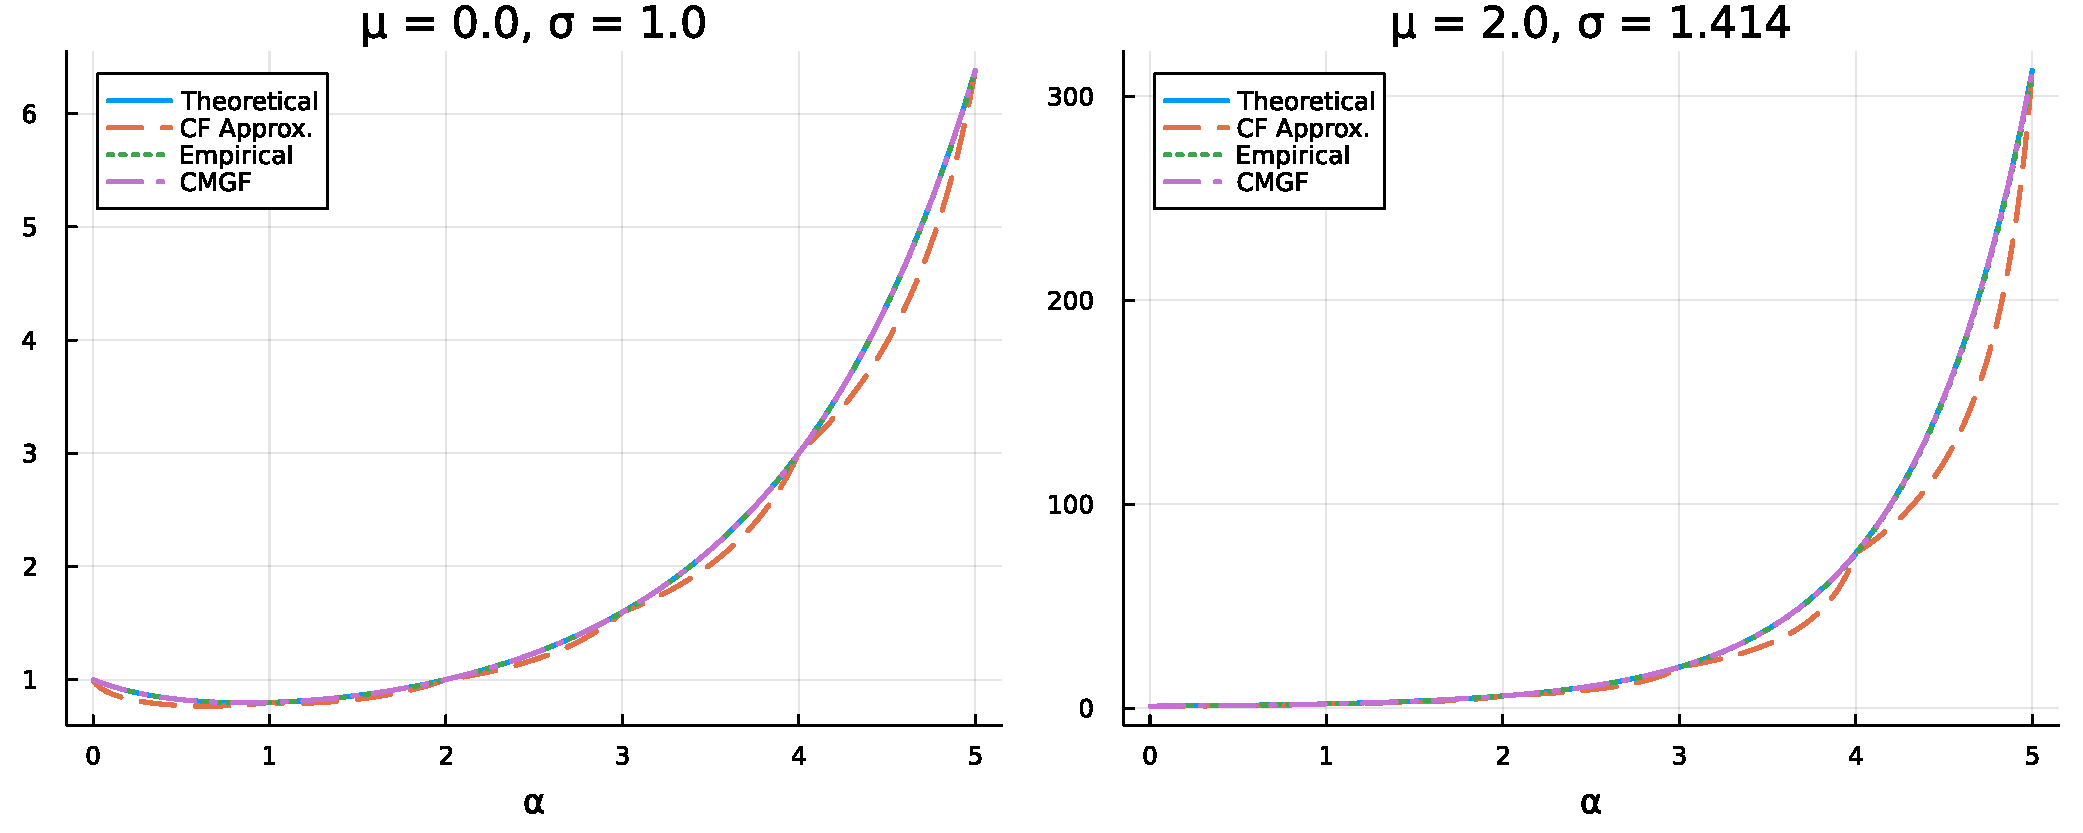
\includegraphics[width=1.1\textwidth]{figures/normal_value_comparison_normal.pdf}
    \caption{Comparison of different fractional moments for the Normal Distribution}
    \label{fig:normal_plot_values}
\end{figure}

The figures above show fractional moment values for various orders \(\alpha\) and different parameter values as computed using the Caputo-Fabrizio MGF, the two accurate MGFs, the CMGF and the empirical method. The results are consistent across all three distributions. The values of the accurate MGFs (blue line), the CMGF (dashed purple line) and empirical values (dashed green-line) almost completely agree, confirming the accuracy and usability of these methods. The values obtained by the Caputo-Fabrizio MGF are always smaller or equal to the values of the accurate MGF expressions. This observation is in line with the result that the errors are always non-negative. Moreover, for all three distributions, an increase in the parameter values, leads to substantially larger fractional moment values. Correspondingly, the errors of the Caputo-Fabrizio MGF also increase, confirming that the approximation error grows with the distribution parameters. 

We obtain the following table, including the run-time (in seconds) of these different methods:
\begin{table}[H]
    \centering 
\begin{tabular}{lccc}
  \toprule
  \textbf{Method} & \textbf{Poisson} & \textbf{Exponential} & \textbf{Normal} \\\midrule
  Theoretical & 0.159 & 0.045 & 0.060 \\
  CF Approx.  & 0.161 & 0.035 & 0.029 \\
  CMGF        & 1.264 & 0.181 & 0.832 \\
  Empirical   & 49.993 & 66.076 & 64.815 \\\bottomrule
\end{tabular}
\caption{Run-time of different methods} 
\label{tab:run_time}
\end{table}
The run-time values reported in table \ref{tab:run_time} are averages over 1000 executions for the theoretical and Caputo-Fabrizio MGFs, 100 executions for the CMGF and 10 executions for the empirical method. Unsurprisingly, the empirical method is the least computationally efficient method, due to the requirement of one million simulated samples. The theoretical and Caputo-Fabrizio MGF methods have comparable run-times, both being highly efficient. The CMGF method is also fast, but noticeably slower than the former two, likely due to the increased complexity of the integrand. The results of the Poisson distribution somewhat differ from those of the Normal and Exponential distribution. This discrepancy may come from  the discrete nature of the Poisson distribution, which requires its moments to be computed in a slightly different numerical manner.

We now focus on the errors of the Caputo-Fabrizio MGF. Specifically, for each of distribution we compute the difference between the theoretical fractional moments: \(\displaystyle \int_{-\infty}^{\infty} x^\alpha  f_X(x) dx\) and those computed by the Caputo-Fabrizio MGF: \(\displaystyle \int_{-\infty}^{\infty}  \frac{x^{n+1} }{(1 - \beta)x + \beta} f_X(x) dx\) for various orders \(\alpha\). This error expression corresponds to the analytical approximation error given in theorem \ref{t: MGF_inaccurate}.
The observant reader might notice that all of the errors in the upcoming sections are non-negative and may incorrectly conclude that these are the absolute or squared errors. This is not the case. Since the expression for the pointwise error function \(E(x, \alpha)\) as in \ref{def:error} is always non-negative, it follows that \( \displaystyle x^\alpha \geq \frac{x^{n+1} }{(1 - \beta)x + \beta}\) and thus \(\displaystyle \int_{-\infty}^{\infty} x^\alpha  f_X(x) dx \geq  \displaystyle \int_{-\infty}^{\infty}  \frac{x^{n+1} }{(1 - \beta)x + \beta} f_X(x) dx\) for any distribution. Thus the approximation error from theorem \ref{t: MGF_inaccurate} is guaranteed to be non-negative.


\subsubsection{Poisson Distribution}
First, we let \(X \sim Poisson(\lambda)\), with the probability mass function defined as in Appendix \ref{s:app_common_distributions}. The Poisson distribution has positive support, thus numerical issues will be avoided. It is not possible to obtain moments of negative order for the Poisson distribution.

\begin{figure}[H]
    \centering
    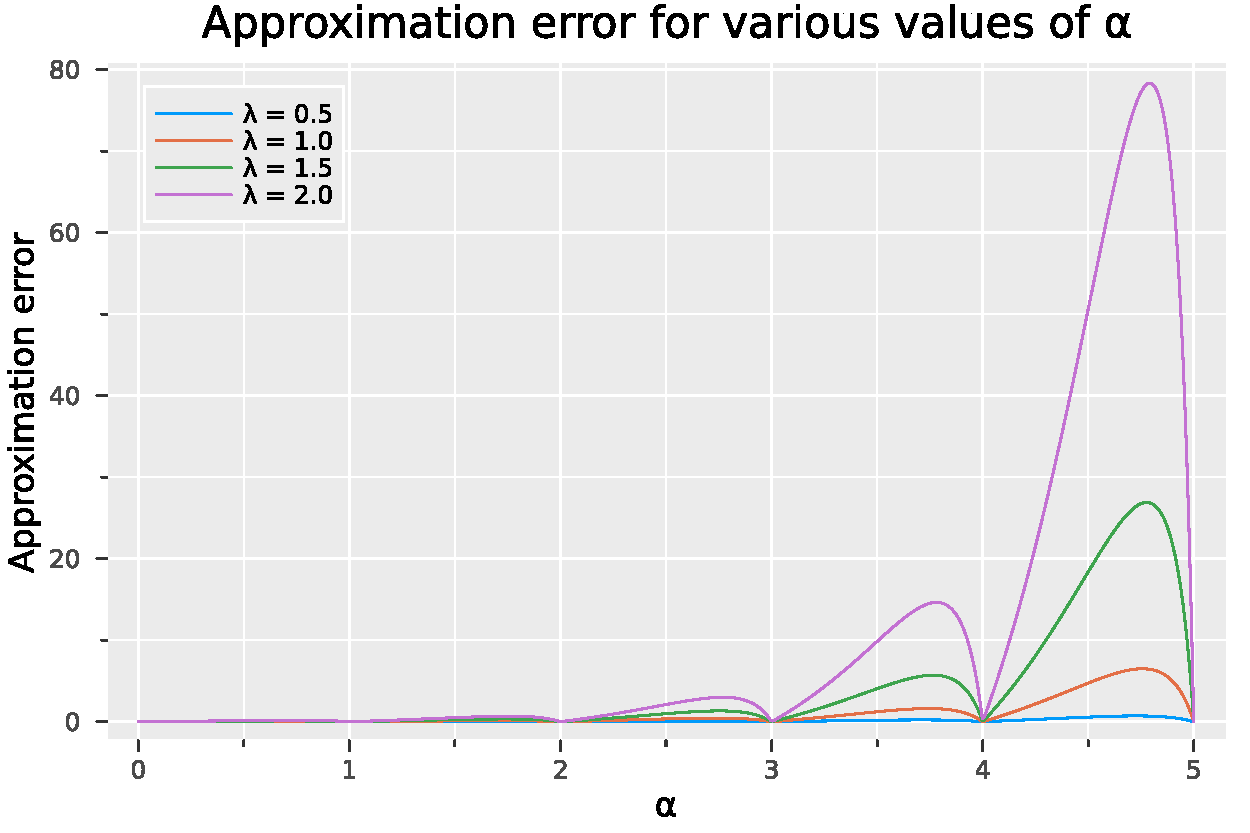
\includegraphics[width=0.65\textwidth]{figures/error_plot_poisson.pdf}
    \caption{Approximation error for the Poisson Distribution}
    \label{fig:poisson_plot_error}
\end{figure}


The trend of the errors in figure \ref{fig:poisson_plot_error} is rather similar to the trend displayed in figure \ref{fig:error_MGF_fixed_x}. That is, the errors behave concavely between each interval of subsequent integers. The plots of the error trends for the Exponential distribution is also very similar. Thus, this plot will not be included. Figure \ref{fig:poisson_plot_error} offers us some additional informational. Namely, the approximation errors increase with the parameter values of the underlying distribution function, in this case the Poisson distribution.


\begin{table}[H]
    \centering
\begin{tabular}{ccccccc}
  \toprule
  \textbf{\(\lambda\)} & \textbf{minimum} & \textbf{maximum} & \textbf{mean} & \textbf{standard deviation} & \textbf{skewness} & \textbf{\(c_v\)} \\\midrule
  0.5 & 0.0 & 0.715 & 0.128 & 0.191 & 1.915 & 1.494 \\
  1.0 & 0.0 & 6.5 & 1.021 & 1.713 & 2.075 & 1.679 \\
  1.5 & 0.0 & 26.904 & 3.895 & 7.001 & 2.176 & 1.797 \\
  2.0 & 0.0 & 78.34 & 10.687 & 20.143 & 2.251 & 1.885 \\\bottomrule
\end{tabular}

\caption{Poisson Distribution - Approximation Error Statistics} 
\label{tab:poisson_error}
\end{table}
The statistics in table \ref{tab:poisson_error} further support this observation.
Both the average and maximum of the errors increase, as the parameter \(\lambda\) grows. Moreover, the standard deviation of the errors also increases and the distribution of the errors tends to become more right-skewed as \(\lambda\) increases. For all values of \(\lambda\), the minimum error is zero, which occurs when \(\alpha \in \mathbb{N}\). In the last column, the coefficient of variation has been reported, which has been given by the formula \(\displaystyle \frac{\sigma}{\mu}\), where \(\mu\) and \(\sigma\) denote the sample mean and sample standard deviation respectively \citep{hendricks1936}. This metric of measurement allows us to objectively compare the variability of the errors of each of the parameter configurations. The lower \(c_v\), the lower the relative variability of the errors. This low variability is something we strive for, as it allows us to describe our data with greater confidence. Once more, this statistic also increases with \(\lambda\). For \(\lambda = 0.5\) we may still be able to obtain reliable results. In contrast, the other configurations are likely to be too unreliable in practice, especially for orders of \(\alpha > 3\).

\subsubsection{Exponential Distribution}
We now consider \(X \sim Exponential(\beta)\), with PDF as defined in Appendix \ref{s:app_common_distributions}.
The support of the Exponential distribution is \([0, \infty)\), thus the integration process will avoid most numerical issues. Moreover, all relevant moments of the Exponential distribution are raw moments, which are precisely the moments we are interested in.
\newline

We obtain the following associated table with some core statistics:
\begin{table}[H]
    \centering
\begin{tabular}{ccccccc}
  \toprule
  \textbf{\(\beta\)} & \textbf{minimum} & \textbf{maximum} & \textbf{mean} & \textbf{standard deviation} & \textbf{skewness} & \textbf{\(c_v\)} \\\midrule
  0.5 & 0.0 & 0.329 & 0.074 & 0.083 & 1.762 & 1.12 \\
  1.0 & 0.0 & 22.119 & 2.907 & 5.612 & 2.314 & 1.93 \\
  1.5 & 0.0 & 225.731 & 25.477 & 54.91 & 2.513 & 2.155 \\
  2.0 & 0.0 & 1128.26 & 115.489 & 265.154 & 2.655 & 2.296 \\\bottomrule
\end{tabular}

\caption{Exponential Distribution - Approximation Error Statistics} 
\label{tab:exp_error}
\end{table}

The results in table \ref{tab:exp_error} align with the conclusions derived from table \ref{tab:poisson_error}. The greater the parameter values and order of \(\alpha\), the greater the (average) approximation error.  An interesting observation is that for \(\beta = 1.5\) the average approximation error exceeds the maximum approximation error for \(\beta = 1.0\). For all values of \(\beta\), the skewness is positive, implying that the distribution of the approximation errors is right-skewed. Thus, clearly the distribution of the errors is not symmetric and therefore certainly not a Normal distribution.  From table \ref{tab:exp_error}, it is clear that the coefficient of variation increases as the parameter \(\beta\) increases. For \(\beta = 0.5\) all result are reasonable. The Caputo-Fabrizio MGF in combination with the Exponential(0.5) could still be viable in practice. For Exponential(1), this conclusion may depend on the maximum order of \(\alpha\).

\subsubsection{Normal Distribution}
We now consider \(X \sim \mathcal{N}(\mu, \sigma)\), with PDF as defined in Appendix \ref{s:app_common_distributions}. This distribution is of particular interest as it has two parameters. Thus, we can analyse the differences of effect of both parameters on the approximation error. Therefore, while raw fractional moments of the Normal distribution are not commonly used in practice, we can still obtain valuable insights from these computations. In order to avoid numerical issues, absolute values have been used to compute the fractional moments.

\begin{figure}[H]
    \centering
    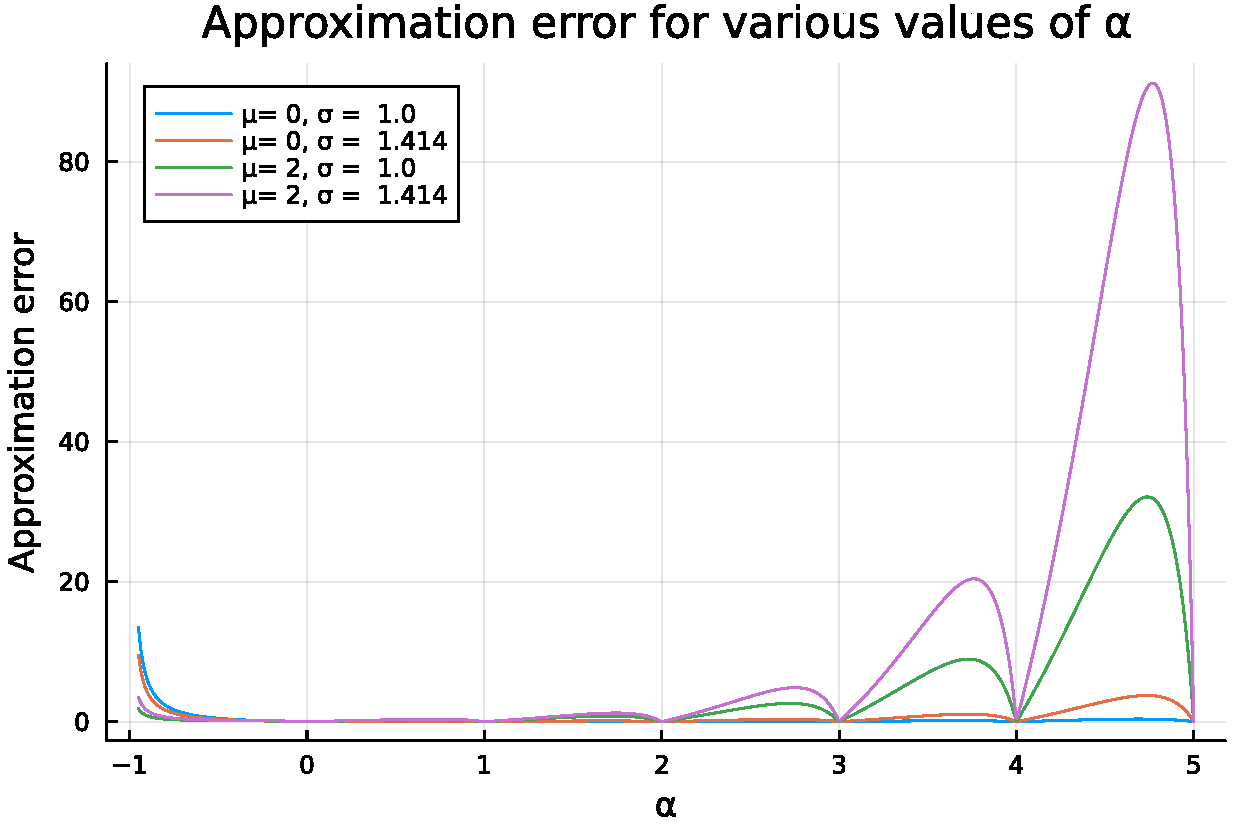
\includegraphics[width=0.675\textwidth]{figures/error_plot_normal.pdf}
    \caption{Approximation error for the Normal Distribution}
    \label{fig:normal_plot_error}
\end{figure}
As illustrated in figure \ref{fig:normal_plot_error}, the approximation error increases with \(\mu\) and \(\sigma\). This result is consitent with the result obtained for the other two distributions. Moreover, this figure also displays the errors for order \(\alpha \in (-0.95, 0)\). Interestingly, for negative orders of \(\alpha\), the effect of the parameter values seems to be the reverse. Larger values of \(\mu\) and \(\sigma\) are associated with smaller approximation errors.
\newline 

We obtain the following associated table with some core statistics:
\begin{table}[H]
    \centering
\begin{tabular}{cccccccc}
  \toprule
  \textbf{\(\mu\)} & \textbf{\(\sigma\)} & \textbf{minimum} & \textbf{maximum} & \textbf{mean} & \textbf{standard deviation} & \textbf{skewness} & \textbf{\(c_v\)} \\\midrule
  0.0 & 1.0 & 0.0 & 13.439 & 0.298 & 1.07 & 7.898 & 3.591 \\
  0.0 & 1.414 & 0.0 & 9.505 & 0.7 & 1.141 & 2.824 & 1.629 \\
  2.0 & 1.0 & 0.0 & 32.123 & 4.517 & 8.055 & 2.269 & 1.783 \\
  2.0 & 1.414 & 0.0 & 91.231 & 11.411 & 22.404 & 2.428 & 1.963 \\\bottomrule
\end{tabular}

\caption{Normal Distribution - Approximation Error Statistics} 
\label{tab:normal_error}
\end{table}
The statistics in table \ref{tab:normal_error} support the visual conclusions drawn from figure \ref{fig:normal_plot_error}. The average of the approximation error for \(\mu = 0\) is acceptable. However, the size of its coefficient of variation compared to the other parameter configurations stands out. Indeed, configuration \((\mu, \sigma) = (0, 1)\) and configuration \((\mu, \sigma) = (0, \sqrt{2})\) have a rather similar standard deviation, however, the latter has approximately twice the average error. Except for this case, \(c_v\) again tends to increase as the parameter values increase, suggesting higher relative variability in approximation errors. Similar to the other distributions, for all parameter-configurations, the distribution of the errors is right-skewed. Thus, the approximation errors of a Normal distribution are not Normally distributed themselves! This result is confirmed in figure \ref{fig:error_histogram}. Even in the histogram of the parameter-configuration with the greatest parameter values, more than 50\% of the approximation errors cluster around zero, with only a small number of observations falling in the range \((40, 80)\). As before, the average errors and variability for large parameters may be too great to be reliable depending on the context of the application.

\begin{figure}[H]
    \centering
    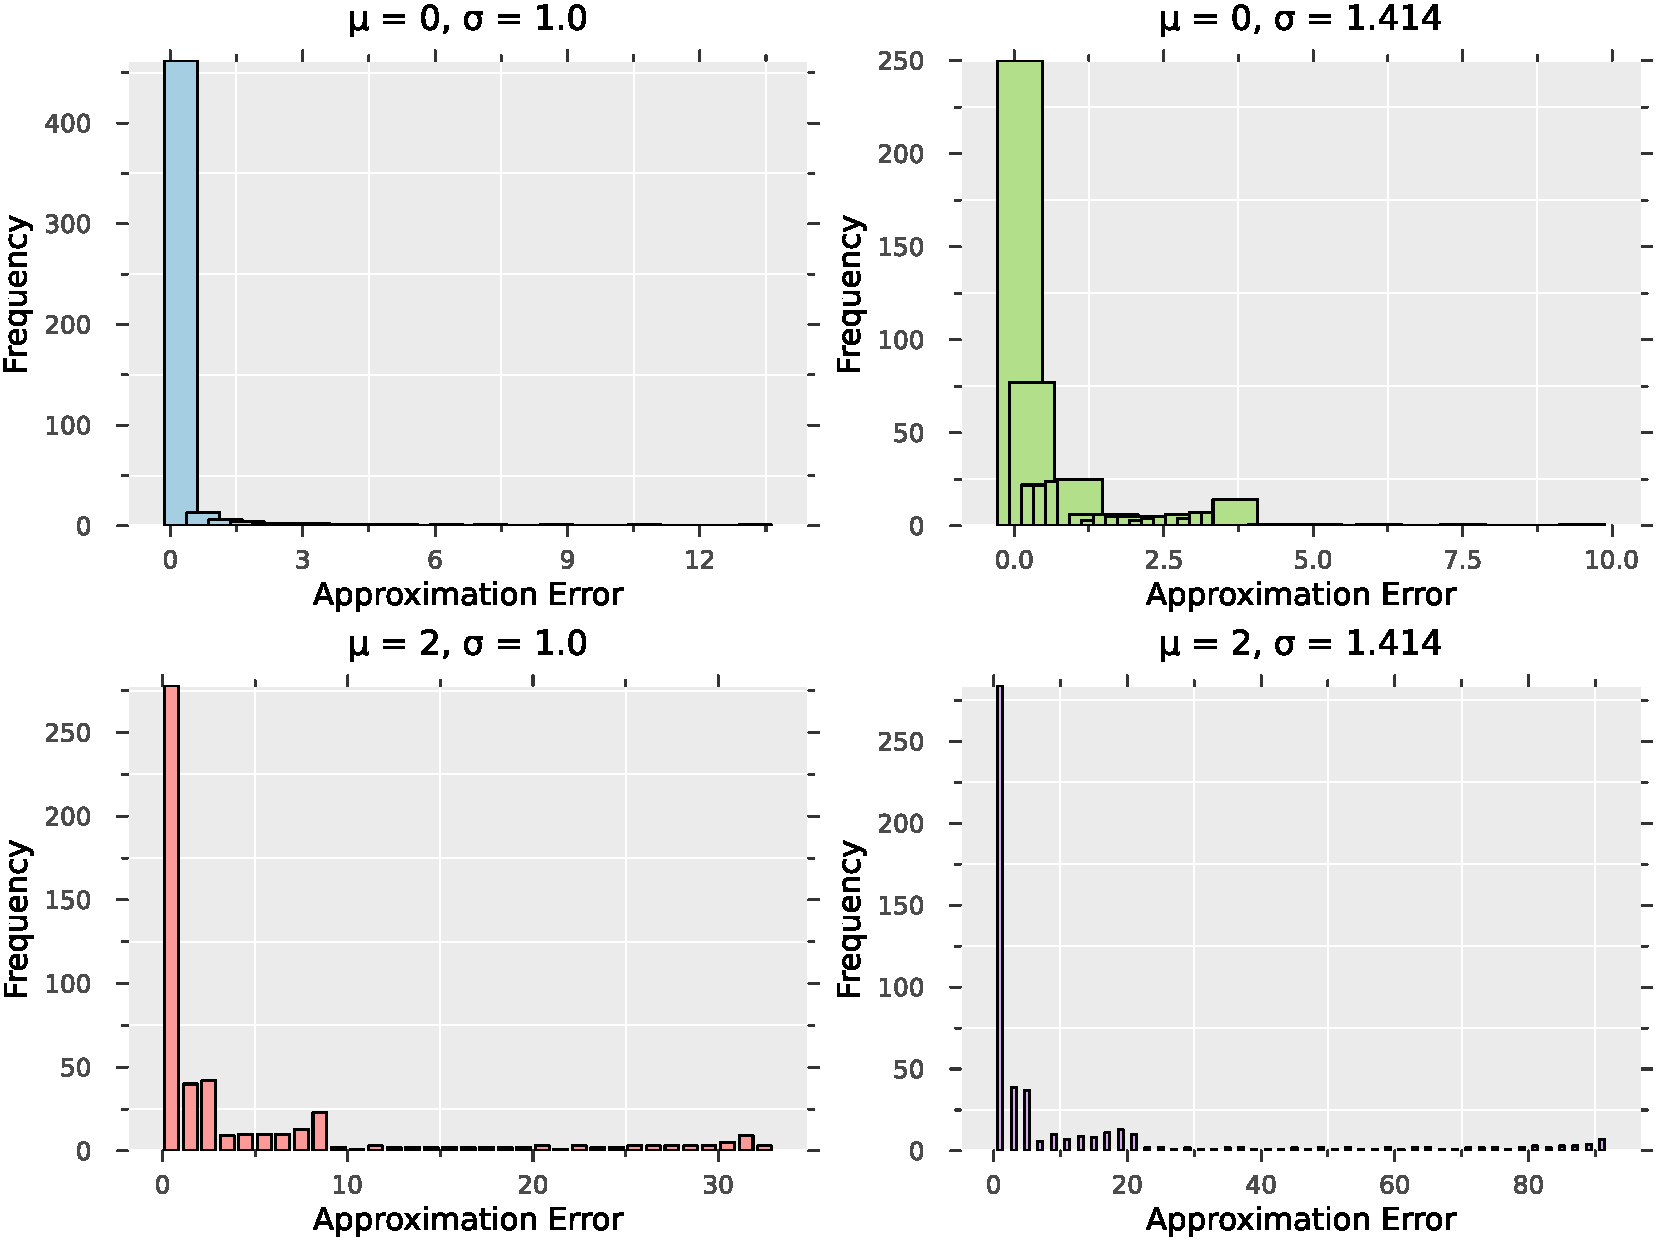
\includegraphics[width=0.83\textwidth]{figures/error_histogram.pdf}
    \caption{Error Histogram for the Normal Distribution}
    \label{fig:error_histogram}
\end{figure}




\subsection{General results}
Based on the three distributions analysed, we arrive at the following  general conclusions:
\begin{itemize}
    \item As the parameter value of the underlying distribution increases, both the average and maximum approximation error tend to increase.
    \item For all distributions considered, higher parameter values, lead to greater standard deviations in the approximation errors.
    \item Furthermore, the coefficient of variation also increases with larger parameter values, indicating that the standard deviation increases at a higher rate than the mean - a stronger result than the increase in the standard deviation alone.
    \item For all considered distributions and parameter values, the distribution of the approximation errors is right-skewed. Thus, we can conclude that the latter does not follow a Normal, or any other symmetric, distribution.
\end{itemize}
These findings raise important considerations regarding the reliability of the Caputo-Fabrizio MGF in practice. While high parameter values often result in a large coefficient of variation, suggesting that the quality of the approximation behaves inconsistently. Figure \ref{fig:error_histogram} offers a different perspective. Namely, in the case of the Normal distribution, at least 50\% of the errors are clustered around zero. Most importantly, in this section, we are considering a sample of approximation errors of 500 fractional moments. When applying moments of fractional order in practice such as in \citet{hansen2024} or \citet{gyzl2013}, one usually computes no more than five or ten moments. Considering the latter, metrics such as the standard deviation and coefficient of variation may not always be relevant or decisive when evaluating the usability of the Caputo-Fabrizio MGF. Therefore, rejecting a parameter configuration solely based on its high variability may be too strict. In general, as long as the fractional order of the moment remains below 3 or is close to an integer, the Caputo-Fabrizio MGF tends to yield sufficiently accurate results. This supports its viability in practical cases, such as in \citet{hansen2024}, where only fractional moments of relatively low order are of interest.